%!TEX root = ../report.tex
\chapter{Hardware Architecture}
\label{ch:hardware}
This section outlines hardware architecture of \ProjectName{RUGSA3}. The first part presents an overview of the system and the second part the decisions ...

\section{Hardware Overview}

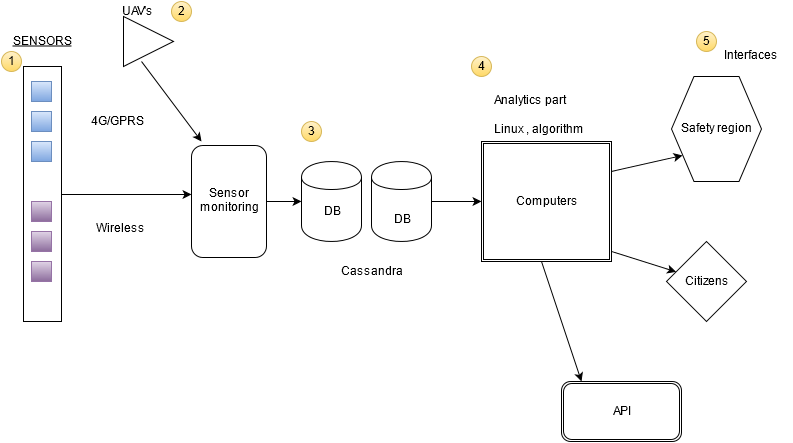
\includegraphics[scale=0.5]{images/HardwareArchitectureOverview.png}

Here is an overview of the System Architecture. Each number corresponds to a decision which will be detailed in the Hardware Design Decision part.


\section{Hardware Design Decisions}
This section defines decisions made regarding the harware selection.

\begin{table}[h]
\begin{tabular}{L{0.2\textwidth} L{0.6\textwidth}}
    \textbf{Name} 			& \textbf{Choice of the computer for data analyze} \\ \toprule
    \textbf{Decision} 		& \textbf{DEC-4}\\ \midrule
    \textbf{Status} 		& \textbf{Approved} \\ \midrule
    \textbf{Problem/Issue} 	& The system needs computer to analyze data from sensors, UAV's ,weather forecast. \\ \midrule
    \textbf{Decision} 		& IBM Supercomputer ...\\ \midrule
    \textbf{Alternatives} 	& \textit{BB}\\
    						& Other brand .\\
    						& \textit{BB}\\
    						& BBBB.\\
    						\midrule
    \textbf{Arguments} 		& IBM supercomputer uses Linux which is the oS we choosed. \\
    						& 	\begin{tabular}{l|lllllll|l}
							& 		\rot{Reliability} & \rot{Resilience} & \rot{Performance} & \rot{Security} & \rot{Scalability} & \rot{Cost} & \rot{\textbf{Score}} \\ \hline
							% 					
								\end{tabular} \\
    \\ \bottomrule
\end{tabular}


\caption{Decision -- Choice of computer}
\label{table:linux}
\end{table}

%Performance , Speed of calculation , Core ; lINUX

\begin{table}[h]
\begin{tabular}{L{0.2\textwidth} L{0.6\textwidth}}
    \textbf{Name} 			& \textbf{Data representation - Interface with the third parties} \\ \toprule
    \textbf{Decision} 		& \textbf{DEC-4}\\ \midrule
    \textbf{Status} 		& \textbf{Approved} \\ \midrule
    \textbf{Problem/Issue} 	& The system needs to interact with the third parties. \\ \midrule
    \textbf{Decision} 		& Dashboard for the emergency services\\ Rack server \\ \midrule
    \textbf{Alternatives} 	& \textit{BB}\\
    						& DRAFT .\\
    						& \textit{BB}\\
    						& BBBB.\\
    						\midrule
    \textbf{Arguments} 		& \\

    \\ \bottomrule
\end{tabular}
\caption{Decision -- Interface with third parties}
\label{table:linux}
\end{table}

